\documentclass[11pt,a4paper]{article}

\usepackage[margin=2.2cm]{geometry}
\usepackage[T1]{fontenc}
\usepackage{lmodern}
\usepackage{microtype}
\usepackage{booktabs}
\usepackage{enumitem}
\usepackage[most]{tcolorbox}
\usepackage{needspace}
\usepackage{capt-of}
\usetikzlibrary{patterns}
\usepackage{hyperref}
% Shared TikZ styles, colours and the running example.
% Used by both slides/slides.tex and notes/lecture.tex.
%
% Running example (X = {a,...,e}, Y = {1,...,5}):
%   edges  a1 a3 | b2 b5 | c4 c5 | d1 d2 | e1
%   Phase 1: shortest aug. path length 1  -> a1, b2, c4
%   Phase 2: shortest aug. path length 3  -> d1 a3
%   Phase 3: shortest aug. path length 5  -> e1 d2 b5   (perfect matching)

\usepackage{amsmath,amssymb,mathtools}
\usepackage{tikz}
\usetikzlibrary{arrows.meta,positioning,calc,fit,backgrounds,decorations.pathreplacing,shapes.geometric}

\definecolor{hkblue}{HTML}{2F5D9B}
\definecolor{hkorange}{HTML}{D1793A}
\definecolor{hkred}{HTML}{C0392B}
\definecolor{hkgreen}{HTML}{2E8B57}
\definecolor{hkgrey}{HTML}{6B6B6B}

\newcommand{\symdiff}{\oplus}
\newcommand{\M}{M}
\newcommand{\bigO}[1]{O\!\left(#1\right)}

\tikzset{
  boy/.style={circle, draw=hkblue!80, fill=hkblue!16, minimum size=6.6mm,
              inner sep=0pt, font=\footnotesize, thick},
  girl/.style={circle, draw=hkorange!90, fill=hkorange!22, minimum size=6.6mm,
               inner sep=0pt, font=\footnotesize, thick},
  freev/.style={draw=hkgreen, line width=1.3pt},   % ring that marks a free vertex
  unm/.style={line width=0.6pt, draw=black!35},          % unmatched edge
  mat/.style={line width=1.9pt, draw=black!80},          % matching edge
  aug/.style={line width=2.2pt, draw=hkred},             % edge on augmenting path
  Medge/.style={line width=1.9pt, draw=hkblue},
  Nedge/.style={line width=1.9pt, draw=hkorange, dashed},
  layerlab/.style={font=\footnotesize\bfseries, text=hkblue!85!black},
}

% ---- the running example --------------------------------------------------
% left column top->bottom: a e d b c ; right column: 3 1 2 5 4   (planar drawing)
\newcommand{\exnodes}{%
  \node[boy]  (xa) at (0, 2.2) {$a$};
  \node[boy]  (xe) at (0, 1.1) {$e$};
  \node[boy]  (xd) at (0, 0.0) {$d$};
  \node[boy]  (xb) at (0,-1.1) {$b$};
  \node[boy]  (xc) at (0,-2.2) {$c$};
  \node[girl] (y3) at (2.8, 2.2) {$3$};
  \node[girl] (y1) at (2.8, 1.1) {$1$};
  \node[girl] (y2) at (2.8, 0.0) {$2$};
  \node[girl] (y5) at (2.8,-1.1) {$5$};
  \node[girl] (y4) at (2.8,-2.2) {$4$};
}
\newcommand{\exedges}{%
  \draw[unm] (xa)--(y1); \draw[unm] (xa)--(y3);
  \draw[unm] (xb)--(y2); \draw[unm] (xb)--(y5);
  \draw[unm] (xc)--(y4); \draw[unm] (xc)--(y5);
  \draw[unm] (xd)--(y1); \draw[unm] (xd)--(y2);
  \draw[unm] (xe)--(y1);
}
% highlight a vertex as free
\newcommand{\freering}[1]{\draw[freev] (#1) circle (4.4mm);}


\hypersetup{colorlinks=true,linkcolor=hkblue,urlcolor=hkblue}
\setlength{\parindent}{0pt}
\setlength{\parskip}{6pt}
\setlist{nosep,leftmargin=1.4em}

% ---- boxes ---------------------------------------------------------------
\newtcolorbox{thm}[1]{enhanced,colback=hkblue!5,colframe=hkblue!70,boxrule=0.5pt,arc=2pt,
  left=6pt,right=6pt,top=5pt,bottom=4pt,title={\small\bfseries #1},
  coltitle=white,attach boxed title to top left={yshift=-2mm,xshift=2mm},
  boxed title style={colback=hkblue,arc=2pt,boxrule=0pt,top=1pt,bottom=1pt}}
\newtcolorbox{board}{enhanced,colback=black!4,colframe=black!70,boxrule=0.6pt,arc=2pt,
  left=6pt,right=6pt,top=5pt,bottom=4pt,title={\small\bfseries On the board},
  coltitle=white,attach boxed title to top left={yshift=-2mm,xshift=2mm},
  boxed title style={colback=black!70,arc=2pt,boxrule=0pt,top=1pt,bottom=1pt}}
\newtcolorbox{ask}{enhanced,colback=hkorange!8,colframe=hkorange,boxrule=0.5pt,arc=2pt,
  left=6pt,right=6pt,top=5pt,bottom=4pt,title={\small\bfseries Ask the class},
  coltitle=white,attach boxed title to top left={yshift=-2mm,xshift=2mm},
  boxed title style={colback=hkorange,arc=2pt,boxrule=0pt,top=1pt,bottom=1pt}}
\newtcolorbox{key}{enhanced,colback=hkred!6,colframe=hkred,boxrule=0.5pt,arc=2pt,
  left=6pt,right=6pt,top=5pt,bottom=4pt,title={\small\bfseries Leave them with},
  coltitle=white,attach boxed title to top left={yshift=-2mm,xshift=2mm},
  boxed title style={colback=hkred,arc=2pt,boxrule=0pt,top=1pt,bottom=1pt}}

\let\oldsection\section\renewcommand{\section}{\Needspace{9\baselineskip}\oldsection}
\newenvironment{pf}{\par\noindent\textbf{Proof.}\ }{\hfill$\square$\par}

% section tag: slides and time
\newcommand{\sectag}[3]{\Needspace{6\baselineskip}\noindent{\small\colorbox{hkblue!12}{\strut\ \textbf{\color{hkblue}#1}\ \ #2\ \ \textit{#3}\ }}\par\vspace{-2pt}}

% ---- tikz helpers ----------------------------------------------------------
% the running example, with extra drawing commands in #2
\newcommand{\exfig}[2][]{\begin{tikzpicture}[scale=0.62,#1]\exnodes\exedges #2\end{tikzpicture}}
\newcommand{\Mbase}{\draw[mat] (xa)--(y1); \draw[mat] (xb)--(y2); \draw[mat] (xc)--(y4);}

\title{\textbf{Understanding the Core of Hopcroft--Karp}\\[2pt]
\large A teaching lecture for slides 8--12: shortest paths, Theorem 2, Corollaries 3 and 4, Algorithm A, and the $\sqrt n$ bound\\[2pt]
\normalsize CS-G526 \quad Aman Pathak}
\author{}\date{}

\begin{document}
\maketitle

\section*{What this document is for}
The 18-minute script tells you \emph{what to say}. This document is for \emph{you understanding it}, so that when someone interrupts you at slide 9 you can answer from the idea and not from memory. It walks through slides 8 to 12 one at a time. For each slide: the question it answers, the idea in plain words, a worked check on our running example, the proof, and the usual confusions. Section 6 adds a second, shorter proof route from the Cornell CS 6820 lecture notes on matchings, built on BFS levels. It ends with a one-page recap and a quiz.

\textbf{Running example} (used everywhere): workers $X=\{a,b,c,d,e\}$, jobs $Y=\{1,2,3,4,5\}$, edges $a1,a3,b2,b5,c4,c5,d1,d2,e1$. The paths we flip, in order, are
\[
P_0=a1,\quad P_1=b2,\quad P_2=c4,\quad P_3=d1\,a3,\quad P_4=e1\,d2\,b5 ,
\]
with lengths $1,1,1,3,5$ (length = number of edges). After the last flip the matching $\{e1,d2,b5,a3,c4\}$ is perfect.

\subsection*{The five words you need}
\begin{itemize}
  \item \textbf{Matching} $M$: edges with no shared vertex. A vertex is \textbf{free} if no edge of $M$ touches it.
  \item \textbf{Augmenting path} for $M$: a path that starts and ends at free vertices and alternates non-$M$, $M$, non-$M$, \dots, non-$M$. So it has one more non-$M$ edge than $M$ edge, and its \textbf{length is always odd}. (It starts in $X$ and ends in $Y$, so the number of edges is odd.)
  \item \textbf{Flip} $P$: $M\oplus P$, i.e.\ swap which edges of $P$ are in $M$. Lemma 1: this is again a matching, one bigger.
  \item \textbf{Symmetric difference} $A\oplus B$: the edges in exactly one of $A,B$. Flipping is $M\oplus P$; flipping twice is $(M\oplus P)\oplus P'$.
  \item \textbf{Theorem 1} (the tool behind everything here): if $M$ is smaller than another matching $N$ by $s-r$ edges, then $M\oplus N$ contains at least $s-r$ \emph{vertex-disjoint} augmenting paths for $M$.
\end{itemize}

\subsection*{Theorem 1, made concrete (we use it on slides 9, 10 and 12)}
Take $M=\{a1,b2,c4\}$ and $N=\{e1,d2,b5,a3,c4\}$, the final perfect matching. Here $r=3$, $s=5$. Look only at edges in exactly one of them (the common edge $c4$ drops out):
\begin{center}
\exfig{\Mbase
  \draw[Medge] (xa)--(y1); \draw[Medge] (xb)--(y2);
  \draw[Nedge] (xa)--(y3); \draw[Nedge] (xe)--(y1); \draw[Nedge] (xd)--(y2); \draw[Nedge] (xb)--(y5);
  \freering{xd}\freering{xe}\freering{y3}\freering{y5}
  \node[font=\scriptsize,anchor=west] at (3.4,1.65) {\textcolor{hkblue}{solid $=M$}, \textcolor{hkorange}{dashed $=N$}};}
\captionof{figure}{$M\oplus N$ splits into two paths: $e\,1\,a\,3$ and $d\,2\,b\,5$. Both start and end with an $N$-edge at a free vertex of $M$ (green rings).}
\end{center}
Every vertex has at most one $M$-edge and one $N$-edge, so every component of $M\oplus N$ has degree at most 2 and alternates $M,N,M,N,\dots$: it is a path or an even cycle. A cycle has equally many of each. A path with one more $N$-edge than $M$-edge is an augmenting path for $M$ (its ends are free, otherwise the end would carry a second $N$-edge or already be matched inside the path). Since $N$ has $s-r$ more edges than $M$ overall, at least $s-r=2$ components must be of this kind. Here we get exactly two, and they are disjoint because they are different components.

\textbf{Remember:} \emph{a bigger matching always hides many disjoint augmenting paths inside its difference with a smaller one.}

% =====================================================================
\section{Slide 8: why shortest paths, and what we must prove}
\subsection*{The question}
The classical algorithm flips one augmenting path per search. On our graph that is five searches. But look at the start: $a1$, $b2$, $c4$ are all augmenting paths and they do not touch. Why pay for three searches when one pass could take all three? \textbf{Can many paths be flipped at once?}

\subsection*{The idea}
Not every collection can be flipped together, so we need a rule that tells us which paths are safe to take together. The rule is: \emph{always take a shortest augmenting path}. The slide then promises three facts:
\begin{enumerate}
  \item $|P_0|\le|P_1|\le|P_2|\le\cdots$ (Theorem 2, Corollary 3).
  \item If $|P_i|=|P_j|$ then $P_i,P_j$ share no vertex (Corollary 4).
  \item The run contains only $O(\sqrt n)$ different lengths (Theorem 3).
\end{enumerate}
Read them as a chain: (1) says the lengths form a staircase going up; (2) says each step of the staircase is a set of non-touching paths, so it can be found together; (3) says the staircase has few steps. A step of the staircase is a \textbf{phase}. The running time is then (number of phases) $\times$ (cost of one phase) $=\sqrt n\cdot O(m)$.

\subsection*{Worked check}
Our lengths are $1,1,1,3,5$. Three steps: $\{P_0,P_1,P_2\}$ of length 1, $\{P_3\}$ of length 3, $\{P_4\}$ of length 5. Three phases, matching the three phase slides later.

\subsection*{Confusions}
\begin{itemize}
  \item \emph{``Shortest'' means fewest edges, not ``found first''.} The rule is a choice we make; the theorems say that choice is what produces a staircase. For an arbitrary choice of augmenting paths nothing guarantees the lengths behave.
  \item \emph{Length 1 is a single edge between two free vertices.} Phase 1 is just ``take edges whose both ends are free''.
\end{itemize}

% =====================================================================
\section{Slide 9: Theorem 2, shortest paths never get shorter}
\begin{thm}{Theorem 2}
Let $P$ be a shortest augmenting path for $M$, and let $P'$ be an augmenting path for $M\oplus P$. Then $|P'|\ge|P|+|P\cap P'|$.
\end{thm}
\subsection*{What it says in plain words}
You flip a shortest path. Whatever augmenting path still exists afterwards is at least as long as the one you just used, and strictly longer if it overlaps with it. Flipping a shortest path therefore can never \emph{create} a shorter way to augment.

\subsection*{The idea of the proof}
\begin{enumerate}
  \item Flip $P$, then flip $P'$. The matching has grown by \textbf{two}: $N=(M\oplus P)\oplus P'$ has $|N|=|M|+2$.
  \item Compare $N$ with the \emph{original} $M$. Since $M\oplus N=P\oplus P'$ (flipping $P$ and $P'$ one after another is the same as taking the symmetric difference of both), Theorem 1 gives \textbf{two disjoint augmenting paths for $M$} inside $P\oplus P'$.
  \item $P$ was a \emph{shortest} augmenting path for $M$, so each of those two paths has at least $|P|$ edges. They are disjoint, so $|P\oplus P'|\ge 2|P|$.
  \item Count $P\oplus P'$ another way: it is both paths minus the shared edges, $|P\oplus P'|=|P|+|P'|-2|P\cap P'|$.
  \item Put (3) and (4) together: $|P|+|P'|-2|P\cap P'|\ge2|P|$, hence $|P'|\ge|P|+2|P\cap P'|\ge|P|+|P\cap P'|$. The paper states the weaker form.
\end{enumerate}

\subsection*{Worked check on the example}
$M=\{a1,b2,c4\}$. The shortest augmenting path is length 3; take $P=d\,1\,a\,3$. After flipping, $M\oplus P=\{d1,a3,b2,c4\}$, and $P'=e\,1\,d\,2\,b\,5$ is augmenting (length 5).
\begin{center}
\begin{tabular}{@{}lll@{}}
\toprule
step & value & check\\\midrule
$P\cap P'$ & $\{d1\}$, size 1 & the shared edge\\
$|P\oplus P'|$ & $\{a1,a3,e1,d2,b2,b5\}$, size $6$ & $=3+5-2\cdot1$\\
two disjoint paths for $M$ & $e\,1\,a\,3$ and $d\,2\,b\,5$ & the two paths of the figure above\\
each has length $3\ge|P|=3$ & so $|P\oplus P'|\ge6=2|P|$ & equality holds\\
conclusion & $|P'|=5\ge 3+2\cdot1$ & equality again\\\bottomrule
\end{tabular}
\end{center}
So the example is tight: the bound is not just a bound, it is exactly attained.

\subsection*{Where the pieces came from}
\begin{itemize}
  \item The ``$+2$'' in the matching size comes from flipping two augmenting paths.
  \item The step ``each has at least $|P|$ edges'' is the only place that uses \emph{shortest}. If $P$ were not shortest the two hidden paths could be shorter than $P$ and the argument collapses. This is why the algorithm insists on shortest.
\end{itemize}

\subsection*{Confusions}
\begin{itemize}
  \item \emph{Why does $P'$ need to be augmenting for $M\oplus P$ and not for $M$?} Because it is what is left \emph{after} the flip: Theorem 2 is about the next path. (It need not even be augmenting for $M$; in the example it is not.)
  \item \emph{Doesn't ``never shorter'' feel obvious?} No. Flipping changes which edges are matched, which can open up new alternating routes. The theorem rules out that the new routes are shorter.
\end{itemize}

% =====================================================================
\section{Slide 10: Corollaries 3 and 4}
\subsection*{Corollary 3: the staircase goes up}
Apply Theorem 2 to $P=P_i$ and $P'=P_{i+1}$. Then $|P_{i+1}|\ge|P_i|+|P_i\cap P_{i+1}|\ge|P_i|$. So
\[
|P_0|\le|P_1|\le|P_2|\le\cdots,
\]
which is our $1,1,1,3,5$.

\subsection*{Corollary 4: equal length means no touching}
\textbf{Statement.} If $|P_i|=|P_j|$ then $P_i$ and $P_j$ have no vertex in common.

\textbf{First, equal length forces no shared edge.} In Theorem 2 with $|P'|=|P|$ we get $|P\cap P'|\le0$.

\textbf{Then, a shared vertex would force a shared edge.} This is the clever step. After $P_i$ is flipped, \emph{every} vertex of $P_i$ is matched, and matched along an edge of $P_i$ (the two ends were free and now have a partner; the inside vertices swapped partner). A later path $P_j$ is augmenting, so its two ends are free; a vertex of $P_i$ is not free, so if $P_j$ goes through it, it goes through it as an \emph{inside} vertex. An inside vertex of an alternating path uses its matching edge. That matching edge is an edge of $P_i$. So $P_i$ and $P_j$ share an edge, which we just excluded.
\begin{center}
\begin{tikzpicture}[x=1.05cm,y=0.9cm]
  \node[font=\scriptsize\bfseries] at (1.5,1.5) {before flipping $P_i$};
  \node[boy] (a1) at (0,0.8) {$x_1$}; \node[girl] (b1) at (1,0.8) {$y_1$};
  \node[boy] (c1) at (2,0.8) {$x_2$}; \node[girl] (d1) at (3,0.8) {$y_2$};
  \draw[lnon] (a1)--(b1); \draw[lmat] (b1)--(c1); \draw[lnon] (c1)--(d1);
  \freering{a1}\freering{d1}
  \node[font=\scriptsize\bfseries] at (1.5,-0.3) {after flipping $P_i$};
  \node[boy] (a2) at (0,-1.0) {$x_1$}; \node[girl] (b2) at (1,-1.0) {$y_1$};
  \node[boy] (c2) at (2,-1.0) {$x_2$}; \node[girl] (d2) at (3,-1.0) {$y_2$};
  \draw[lmat] (a2)--(b2); \draw[lnon] (b2)--(c2); \draw[lmat] (c2)--(d2);
  \node[boy] (o) at (3,-2.4) {$x'$};
  \draw[lred,dashed] (o)--(d2);
  \node[font=\scriptsize,hkred,anchor=west] at (3.4,-1.7) {a later path through $y_2$};
\end{tikzpicture}
\captionof{figure}{$y_2$ was a free end of $P_i$. Afterwards it is matched to $x_2$. Any later augmenting path that visits $y_2$ must continue along $y_2x_2$, an edge of $P_i$.}
\end{center}

\subsection*{A technical gap, honestly}
Theorem 2 compares only \emph{consecutive} paths $P_i,P_{i+1}$ (the second is augmenting for the matching after the first). Corollary 4 is about any two with equal length, maybe far apart. The paper closes the gap: take the equal-length pair that touches and has the smallest distance between them. Everything in between has the same length (by Corollary 3) and is disjoint from both, so $P_j$ is still augmenting right after $P_i$, and Theorem 2 applies. If someone asks, that is the answer.

\subsection*{Worked check}
$P_0,P_1,P_2$ (length 1): $a1,b2,c4$ share no vertex. OK. $P_3=d1a3$ and $P_4=e1d2b5$ \emph{do} share vertices ($d$, $1$), and indeed their lengths differ, $3\ne5$. OK.

\subsection*{What we gain}
The sequence splits into blocks of equal length; within a block the paths are pairwise disjoint, so their order does not matter and we can look for them together.

% =====================================================================
\section{Slide 11: Algorithm A}
\begin{thm}{Algorithm A}
\textbf{Step 0.} $M\gets\emptyset$.\quad
\textbf{Step 1.} Let $\ell$ be the length of a shortest augmenting path. Find a \emph{maximal} set $\{Q_1,\dots,Q_t\}$ of vertex-disjoint augmenting paths of length $\ell$. If there is no augmenting path, stop.\quad
\textbf{Step 2.} Flip all of them; go to Step 1.
\end{thm}
\subsection*{Is it legal to flip a whole set at once?}
Yes. The $Q_i$ share no vertex, so flipping one does not disturb the others: each is still augmenting for the changing matching, each is still of length $\ell$ (lengths cannot drop, by Theorem 2), and each adds one edge. Flipping a disjoint set of $t$ paths is therefore the same as $t$ single shortest-path flips in a row. So everything proved about the shortest-path sequence still holds.

\subsection*{Is it correct?}
It stops only when no augmenting path exists, and by Berge (Corollary 1) that means $M$ is maximum.

\subsection*{Maximal vs.\ maximum}
\textbf{Maximal}: nothing can be added. \textbf{Maximum}: the largest possible. Algorithm A needs only maximal.
\begin{center}
\exfig{\Mbase \draw[aug] (xd)--(y1)--(xa)--(y3); \node[font=\scriptsize] at (1.4,-3.2) {order 1: $\{d1a3\}$, 1 path};}\qquad
\exfig{\Mbase \draw[aug] (xe)--(y1)--(xa)--(y3); \draw[aug] (xd)--(y2)--(xb)--(y5); \node[font=\scriptsize] at (1.4,-3.2) {order 2: $\{e1a3,\,d2b5\}$, 2 paths};}
\captionof{figure}{Phase 2 ($M=\{a1,b2,c4\}$, $\ell=3$). Both sets are maximal; only the second is maximum. Thick black $=M$, red $=$ the paths.}
\end{center}
In the first set, adding $e1a3$ fails ($a$ and $3$ are used), adding $d2b5$ fails ($d$ is used), so it is maximal even though a bigger choice exists. Phase 1 is the same story: $\{a1,b2,c4\}$ is maximal (every other edge touches a used vertex), though a maximum matching has five edges. Finding a \emph{maximum} set would be a harder problem in itself, and we do not need it.

\subsection*{Why $\ell$ grows after every phase}
Suppose after the phase a path $R$ of length $\ell$ were still augmenting. Then $R$ is the same length as the $Q_i$ and comes after them in a shortest-path run, so Corollary 4 says $R$ shares no vertex with any $Q_i$. But then we could have added $R$ to our set, contradicting maximality. So the next shortest path is strictly longer than $\ell$. Since lengths are odd, it is at least $\ell+2$.

\subsection*{Confusions}
\begin{itemize}
  \item \emph{Does the choice inside a phase change the result?} It changes which paths we flip and how big the matching is afterwards (see the figure), not the validity or the phase bound.
  \item \emph{Where is the hard work hidden?} In ``find a maximal set''. Slides 13 to 16 show it is done in $O(m+n)$ by BFS plus DFS.
\end{itemize}

% =====================================================================
\section{Slide 12: why only about $\sqrt n$ phases}
\subsection*{The question}
A phase is cheap. But if there were $n$ phases we would gain nothing over the classical $O(mn)$. How many are there?

\subsection*{The two facts, and why neither is enough alone}
\begin{enumerate}
  \item Every phase makes the shortest augmenting path \textbf{longer}. Lengths are odd, so it grows by at least 2: $1,3,5,7,\dots$
  \item Every phase adds \textbf{at least one pair} to the matching.
\end{enumerate}
Fact 2 alone gives only ``at most $n/2$ phases'', which is useless. Fact 1 is what helps, because of one sentence:

\begin{key}A long augmenting path uses up many vertices, and the graph has only $n$ vertices. So there cannot be many long paths that are disjoint.\end{key}
Short paths get used up quickly (each phase pushes the length up); long paths cannot be numerous (they do not fit). Count the phases in two stages.

\subsection*{Step 1: after $\sqrt n$ phases, the shortest path is long}
Lengths are odd and strictly increase from phase to phase, so each phase adds at least 2. Phase 1 has length $\ge1$, phase $k$ has length $\ge2k-1$. Once $\sqrt n$ phases are done, the next shortest augmenting path has length $\ge2\sqrt n+1$.

\subsection*{Step 2: few such paths exist}
Let $r$ be the current size and $s$ the size of a maximum matching. By Theorem 1 there are $s-r$ disjoint augmenting paths for the current matching. Each is at least as long as the shortest one, so each has $\ge2\sqrt n+1$ edges, i.e.\ $\ge2\sqrt n+2$ vertices. They are disjoint and the graph has only $n$ vertices:
\[
(s-r)\,(2\sqrt n+2)\ \le\ n\quad\Longrightarrow\quad s-r\ \le\ \frac{n}{2\sqrt n}=\tfrac12\sqrt n .
\]
\begin{center}
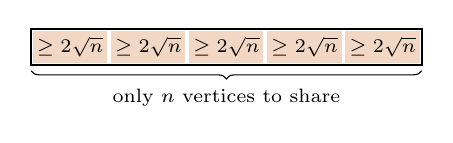
\begin{tikzpicture}[x=0.62cm,y=0.5cm]
  \draw[thick] (0,0) rectangle (8,0.9);
  \foreach \i in {0,1,2,3,4}{
    \fill[hkorange!30] (1.6*\i+0.04,0.04) rectangle (1.6*\i+1.56,0.86);
    \node[font=\scriptsize] at (1.6*\i+0.8,0.45) {$\ge2\sqrt n$};}
  \draw[decorate,decoration={brace,mirror,amplitude=3pt}] (0,-0.15)--(8,-0.15) node[midway,below=3pt,font=\scriptsize]{only $n$ vertices to share};
\end{tikzpicture}
\captionof{figure}{Disjoint long paths are packed into $n$ vertices: at most $\frac12\sqrt n$ fit.}
\end{center}

\subsection*{Step 3: so few phases remain}
We are $s-r\le\tfrac12\sqrt n$ pairs short, and every phase adds at least one pair. So at most $\tfrac12\sqrt n$ more phases.

\subsection*{Total}
$\sqrt n+\tfrac12\sqrt n=\tfrac32\sqrt n=O(\sqrt n)$ phases. (The paper's careful count is $2\lfloor\sqrt s\rfloor+2$.)

\subsection*{The argument with real numbers: $n=100$}
\begin{itemize}
  \item \textbf{Stage 1.} $\sqrt n=10$, so run 10 phases. Just count them: 10 phases.
  \item After that the shortest augmenting path has length $\ge21$, so it has at least 22 vertices.
  \item Suppose $k$ pairs are still missing. There are $k$ disjoint augmenting paths (Theorem 1), each with $\ge22$ vertices. Five of them would need $5\cdot22=110>100$ vertices, which do not exist. So $k\le4$.
  \item \textbf{Stage 2.} Each phase adds at least one pair, so at most 4 more phases.
\end{itemize}
Total: at most $10+4=14$ phases, against up to 50 separate searches for the classical algorithm. (The formula gives $\frac32\sqrt{100}=15$.)

\subsection*{Why $\sqrt n$ and not some other cut-off?}
Stop Stage 1 after $t$ phases instead. Stage 1 costs $t$ phases. In Stage 2 the shortest path has length about $2t$, so at most $n/(2t)$ pairs are missing, hence at most $n/(2t)$ more phases. The total is at most $t+\frac n{2t}$: two costs to balance. For $n=100$:
\begin{center}
\begin{tabular}{@{}rrrr@{}}
\toprule
$t$ & Stage 1 phases & Stage 2: at most $n/(2t)$ & total\\\midrule
1 & 1 & 50 & 51\\
5 & 5 & 10 & 15\\
7 & 7 & 7.1 & about 14 (best)\\
10 & 10 & 5 & 15\\
25 & 25 & 2 & 27\\
50 & 50 & 1 & 51\\\bottomrule
\end{tabular}
\end{center}
A small $t$ leaves Stage 2 huge; a large $t$ makes Stage 1 itself huge. The two are equal at $t=\sqrt{n/2}\approx7$, which is of order $\sqrt n$. That is the only reason $\sqrt n$ appears. (We took $t=\sqrt n$ for a clean proof; the constant is slightly worse, $\frac32\sqrt n$ instead of $\sqrt2\sqrt n$, but the order is the same.)

\textbf{One-line version for the class:} short paths get used up quickly because each phase pushes the length up, and long paths cannot be numerous because they do not fit in $n$ vertices.

\subsection*{How big a win is it?}
\begin{center}
\begin{tabular}{@{}rrr@{}}
\toprule
$n$ & classical: up to $n/2$ searches & Hopcroft--Karp: at most $\frac32\sqrt n$ phases\\\midrule
$10$ (our example) & $5$ & $\le 4.7$ (we used 3)\\
$10^4$ & $5{,}000$ & $\le150$\\
$10^6$ & $500{,}000$ & $\le1{,}500$\\\bottomrule
\end{tabular}
\end{center}
Each search and each phase costs $O(m)$-ish, so on a million vertices the number of passes over the graph drops by a factor of more than 300.

\subsection*{Confusions}
\begin{itemize}
  \item \emph{Does the $\sqrt n$ bound count flips or phases?} Phases. Many flips happen inside a phase, for free.
  \item \emph{Why ``at least one pair per phase''?} A phase starts by finding a shortest augmenting path, so there is at least one, and flipping it gains one.
  \item \emph{Is the bound tight?} It is a worst case. Real graphs usually finish in far fewer phases.
\end{itemize}

% =====================================================================
% =====================================================================
\section{A second route: the level-graph proof (Cornell CS 6820)}
Slides 9 to 11 follow the paper: Theorem 2, then Corollaries 3 and 4, then Algorithm A. The Cornell lecture notes on matchings (\href{https://www.cs.cornell.edu/courses/cs6820/2024fa/handouts/matchings.pdf}{CS 6820, Fall 2024, \S1.4}) prove the same result by a different and shorter route, using \emph{distance labels from a BFS}. It is worth knowing, because it explains \emph{why} the lengths grow in a way you can see on a picture, and it is the same BFS you use on slides 13 to 16. In their words, the waste of the classical algorithm is that it ``chooses one augmenting path in each iteration, even if it finds many augmenting paths in the process of searching''.

\subsection*{The residual graph and the levels}
Write $L=X$ (workers) and $R=Y$ (jobs). Build the directed graph $G_M$: orient every edge \textbf{not} in $M$ from $L$ to $R$, and every edge of $M$ from $R$ to $L$. Then (their Lemma 3) \emph{augmenting paths are exactly the directed paths from a free vertex of $L$ to a free vertex of $R$}, because a directed path alternates ``non-$M$ forward, $M$ backward'' automatically. So finding one is just BFS.

BFS from all free vertices of $L$ gives every vertex a label $d(v)$, its distance from the nearest free worker (or $\infty$ if unreachable). An edge $(u,v)$ is \textbf{advancing} if $d(v)=d(u)+1$ and \textbf{retreating} if $d(v)\le d(u)$. (It can never have $d(v)>d(u)+1$, since going through $u$ already reaches $v$ in $d(u)+1$ steps.) The shortest augmenting length is $\ell=\min\{d(v):v\in R\text{ free}\}$.

\textbf{On the example}, phase 2, $M=\{a1,b2,c4\}$, free workers $d,e$:
\begin{center}
\begin{tabular}{@{}lcccccccccc@{}}
\toprule
vertex & $d$ & $e$ & $1$ & $2$ & $a$ & $b$ & $3$ & $5$ & $c$ & $4$\\
$d(v)$ & 0 & 0 & 1 & 1 & 2 & 2 & 3 & 3 & $\infty$ & $\infty$\\\bottomrule
\end{tabular}
\end{center}
Advancing edges: $d\!\to\!1,\ d\!\to\!2,\ e\!\to\!1,\ 1\!\to\!a,\ 2\!\to\!b,\ a\!\to\!3,\ b\!\to\!5$. Retreating: $c\!\to\!5$ and $4\!\to\!c$ (they hang off the unreachable $c$, and are never on a path from a free worker). So $\ell=3$, and these levels are exactly the picture on slide 14.

\subsection*{Blocking set = our ``maximal set of disjoint shortest paths''}
Their \textbf{blocking set} is a \emph{maximal} set of vertex-disjoint \emph{advancing} augmenting paths: the same ``maximal, not maximum'' idea as slide 11. (A small difference: they allow any advancing path that ends at a free job, even one at a level beyond $\ell$; the paper takes only length $\ell$. Both versions work, and on our example there is no difference.) They compute it exactly like slide 16: BFS for the advancing edges, then a DFS with deletion, and they bound the cost by $O(m+n)$ with three observations: deleted vertices are never reinserted, the found paths are disjoint so their lengths add up to at most $n$, and every other loop step pushes or pops a vertex, each vertex at most once.

\subsection*{Their proof that the length grows (their Lemma 6)}
After flipping the blocking set $Q=P_1\cup\dots\cup P_k$, consider the new residual graph $G_{M'}$. Every edge of $Q$ has been \textbf{reversed}; every other edge kept its direction. So every edge $(x,y)$ of $G_{M'}$, measured with the \emph{old} labels $d$, is one of
\begin{enumerate}
  \item a \textbf{reversed} edge of $Q$: $d(y)=d(x)-1$;
  \item an \textbf{advancing} edge not in $Q$: $d(y)=d(x)+1$;
  \item a \textbf{retreating} edge not in $Q$: $d(y)\le d(x)$.
\end{enumerate}
In all three cases \emph{$d$ goes up by at most 1 per edge}. Now take any augmenting path $P$ for $M'$. It starts at a free worker ($d=0$) and ends at a free job ($d\ge\ell$), and the ends were also free before the flip. Since $d$ rises by at most 1 per edge, $P$ has at least $\ell$ edges. To have \emph{exactly} $\ell$ edges, \emph{every} edge must raise $d$ by exactly 1, so $P$ consists only of advancing edges that are not in $Q$. Two cases, both impossible:
\begin{itemize}
  \item $P$ shares no vertex with $Q$: then $P$ could have been added to the blocking set. That contradicts \emph{maximality}.
  \item $P$ shares a vertex $w$ with $Q$: the ends of $P$ are free, but every vertex of $Q$ is now matched, so $w$ is in the middle of $P$, and $P$ must use the matching edge at $w$, which is an edge of $Q$. But $P$ has no edge of $Q$. Contradiction. (This is exactly the ``shared vertex forces shared edge'' step of Corollary 4.)
\end{itemize}
So every augmenting path now has \emph{more} than $\ell$ edges.

\textbf{On the example.} Flip $Q=\{d1a3\}$ in phase 2. The edges $d\!\to\!1,\ 1\!\to\!a,\ a\!\to\!3$ reverse into $1\!\to\!d,\ a\!\to\!1,\ 3\!\to\!a$, each going \emph{down} one level ($1\to0$, $2\to1$, $3\to2$). The new augmenting path is $e\to1\to d\to2\to b\to5$ with old labels $0,1,0,1,2,3$. It must climb from 0 to 3, but the reversed edge $1\!\to\!d$ gives one level back, so it needs two extra edges: $5=3+2\cdot1$. This is the same ``$|P'|\ge|P|+2|P\cap P'|$'' as Theorem 2, seen as a picture: \emph{each reversed edge you are forced to reuse costs two extra steps.}

\subsection*{Their count of phases (their Lemmas 5 and 7)}
\textbf{Lemma 5.} If $M^*$ is a maximum matching and $k=|M^*|-|M|$, then $M\oplus M^*$ has $k$ vertex-disjoint augmenting paths (Theorem 1 again), so some augmenting path has length less than $n/k$: $k$ disjoint paths cannot all be longer than $n/k$ inside only $n$ vertices. \emph{Check:} on the example, $M=\{a1,b2,c4\}$, $k=2$, $n=10$: there is a path shorter than $10/2=5$, and indeed the shortest has length 3.

\textbf{Lemma 7.} Fewer than $2\sqrt n$ phases. \emph{Proof.} Two measures of progress: the matching grows by at least 1 each phase, and the shortest length grows by at least 1 each phase (Lemma 6). After $\sqrt n$ phases the shortest length is $>\sqrt n$, so by Lemma 5, $n/k>\sqrt n$, i.e.\ $k<\sqrt n$ pairs are missing. Each remaining phase adds a pair, so fewer than $\sqrt n$ more phases. Total $<2\sqrt n$.

\textbf{How this relates to slide 12.} It is the same two-stage argument. Slide 12 gets a smaller constant ($\frac32\sqrt n$) because it also uses that lengths are odd, so the length grows by at least \emph{2} per phase, not 1. Both give $O(\sqrt n)$.

\subsection*{Dictionary between the two sources}
\begin{center}
\begin{tabular}{@{}p{4.1cm}p{4.7cm}p{5.2cm}@{}}
\toprule
\textbf{Paper / our slides} & \textbf{Cornell notes} & \textbf{Where}\\\midrule
workers $X$, jobs $Y$ & $L$, $R$ & --\\
Lemma 1 & Lemma 1, Lemma 4 (many disjoint paths) & slide 6\\
Berge, Theorem 1 & Lemma 2, Lemma 5 & slides 7, 9, 12\\
Theorem 2 + Cor.\ 3 + Cor.\ 4 & Lemma 6 (one argument, via $d$) & slides 9, 10, 11\\
maximal set of shortest disjoint paths & blocking set (advancing paths) & slide 11\\
levels, BFS, DFS with deletion & $d(v)$, advancing edges, Algorithm 2 & slides 13 to 16\\
Theorem 3, Corollary 5 & Lemma 7 & slide 12\\\bottomrule
\end{tabular}
\end{center}
Their notes also confirm the timeline entry on slide 18: Edmonds' 1965 paper ``Paths, Trees, and Flowers'' gave the first polynomial algorithm for an augmenting path in general graphs, in $O(mn)$ time, so $O(mn^2)$ for a maximum matching.

\textbf{Which route to use?} On the slides, stay with the paper (it is what we cite). If someone asks ``is there a simpler way to see that the length grows?'', answer with the level-graph picture: \emph{the labels go up by at most 1 per edge, a path of length exactly $\ell$ would have to use only untouched advancing edges, and maximality forbids that.}

\section{The five slides in one picture}
\begin{center}
\fbox{\parbox{0.92\linewidth}{
\textbf{8.}\ Flip shortest augmenting paths, and hope for a staircase of lengths.\\
\textbf{9.}\ Theorem 2: after flipping a shortest path, nothing shorter appears. \emph{(Two paths flipped $\Rightarrow$ Theorem 1 gives two disjoint ones for the old $M$ $\Rightarrow$ count edges.)}\\
\textbf{10.}\ So the lengths go up (Cor.\,3), and equal lengths never touch (Cor.\,4). \emph{(Touching means sharing a matched edge.)}\\
\textbf{11.}\ So each step of the staircase can be found together: a maximal disjoint set. The next step is longer, by maximality.\\
\textbf{12.}\ The staircase has $O(\sqrt n)$ steps: long paths do not fit, and each step gains $\ge1$.\\[2pt]
\textbf{Result:} $O(\sqrt n)$ phases $\times$ $O(m+n)$ per phase.}}
\end{center}

\section{Test yourself}
\begin{enumerate}[label=\textbf{Q\arabic*.},leftmargin=2.4em,itemsep=6pt]
\item Why are augmenting-path lengths always odd?
\item On the example, after $P_3=d1a3$, which augmenting paths exist? (There is exactly one.) Check Theorem 2 on it.
\item In the proof of Theorem 2, which single step fails if $P$ is not a shortest augmenting path?
\item Why can a later augmenting path not pass through a vertex of $P_i$ as one of its \emph{ends}?
\item Give a graph with a maximal set of disjoint shortest augmenting paths that is not maximum. (Use the figure on slide 11.)
\item If we replaced ``maximal'' with ``any non-empty set'' in Step 1, which claim breaks?
\item Show the bound $s-r\le\frac12\sqrt n$ if the shortest path had length at least $3\sqrt n$ instead.
\item In the level-graph proof, why can $d$ rise by at most 1 along any edge of $G_{M'}$? Which edges lower it?
\item On the example, $M=\{d1,a3,b2,c4\}$ after phase 2. Compute $d(v)$ for the new residual graph and read off the shortest augmenting length.
\end{enumerate}

\subsection*{Answers}
\begin{enumerate}[label=\textbf{A\arabic*.},leftmargin=2.4em,itemsep=6pt]
\item It begins at a free vertex of $X$ and ends at a free vertex of $Y$, and the path alternates sides, so it has an odd number of edges.
\item After flipping $P_3$, $M=\{d1,a3,b2,c4\}$ and the only augmenting path is $e\,1\,d\,2\,b\,5$, length 5. Theorem 2: $5\ge3+|P_3\cap P_4|=3+1$.
\item ``Each of the two disjoint paths for $M$ has length at least $|P|$.''
\item Its ends are free; every vertex of $P_i$ is matched after the flip.
\item Phase 2: $\{d1a3\}$ is maximal; $\{e1a3,d2b5\}$ is bigger.
\item The length might not increase after a phase: a path of length $\ell$ could remain, so the phase count bound fails (Step 1 of slide 12).
\item $(s-r)(3\sqrt n)\le n$ gives $s-r\le\frac13\sqrt n$.
\item Edges not in $Q$ keep their direction and were already advancing or retreating ($d$ up by 1 or not up); edges of $Q$ were advancing and are now reversed, so $d$ goes \emph{down} by 1. Reversed edges are the only ones that lower it.
\item Free worker: $e$ only. $d(e)=0$, $d(1)=1$, $d(d)=2$ (via the matched edge $1\!\to\!d$), $d(2)=3$, $d(b)=4$, $d(5)=5$. The free job $5$ is at level 5, so the shortest augmenting length is 5.
\end{enumerate}

\end{document}
